\section{Materials and Methods}
\label{sec:MatMeth}

% ----------------------------------------------------------------------- %
% ----------------------------------------------------------------------- %
\subsection{Study Area}
\label{sec:studyarea}

The German federal state Rhineland-Palatinate (RLP) is located in the western part of Germany and borders Luxembourg, France and Belgium (figure \ref{fig:Study Area}). With 42.3\% (appr. 8400 km$^2$) of the entire state area (19850 km$^2$) covered by forest, RLP is one of the two states with the highest forest coverage among all federal states of Germany \citep{bwi3}. \added{The forest area of RLP is divided into three ownership classes, i.e. state forest (27\%), communal forest (46\%) and privately owned forest (27\%).} The most frequent tree species in RLP are European beech (\textit{Fagus sylvatica}, 21.8\%), oak (\textit{Quercus petrea} and \textit{Quercus robur}, 20.2\%), Norway spruce (\textit{Picea abies}, 19.5\%), Scots pine (\textit{Pinus sylvestris}, 9.9\%), Douglas fir (\textit{Pseudozuga menziesii}, 6.4\%), European larch (\textit{Larix decidua}, 2.4\%) and Silver fir (\textit{Abies alba}, 0.7\%). The share of broadleaf tree species is 58.7\%. The forests of RLP further exhibit heterogeneous structures \citep{bwi3}: around 82\% of the forest area in RLP are mixed forest stands (i.e. at least two different tree species occur in the same stand) and 69\% of the forest area exhibit a multi-layered vertical structure. While the average tree age is around 80 years, most of the forest area (20\%) is occupied by trees between 40 and 60 years of age, whereas 27\% of the trees are older than 100 years. Spatially variable climate conditions have a strong influence on the local growth dynamics as well as tree species composition and create a large variety of forest structures, ranging from characteristic oak coppices (Moselle valley), pure spruce, beech and Scots pine forests (e.g. Hunsr{\"u}ck and Palatinate forest) to mixed forests comprising variable proportions of oak, larch, spruce, Scots pine and beech. Accordingly, RLP has been divided into 16 bioclimatic growing regions that form homogeneous areas with respect to the afore mentioned characteristics \citep{gauer2005}.

\begin{figure}[h]
\centering
\resizebox{1\hsize}{!}{\includegraphics*{terr_sampledesign_bw.png}}
\caption{Spatial distribution of the \bwi{} cluster samples over Rhineland-Palatinate}
\label{fig:Study Area}
\end{figure}

% ----------------------------------------------------------------------- %
% ----------------------------------------------------------------------- %
\subsection{Terrestrial Inventory Data}
\label{sec:terrdata}
The German National Forest Inventory (NFI) is carried out over the entire forest area of Germany in reoccurring time periods of 10 years. The most recent inventory (\bwi{}) has been conducted in the years 2011 and 2012. In this framework, Rhineland-Palatinate is covered by a 2x2 km grid that defines the sample locations for the terrestrial survey. A sample unit consists of four sample locations (also referred to as \textit{sample plots}) that are arranged in squares (so called \textit{clusters}) with a side length of 150 metres (figure \ref{fig:Study Area}). The number of plots per cluster can however vary between 1 and 4 depending on forest/non-forest decisions on the plot level \citep{bwi3_aufn}. In the field survey of the \bwi{}, sample trees for timber volume estimations are selected according to the angle count sampling technique \citep{bitterlich1984}, using a basal area factor ($BAF$) of 4 that is respectively adjusted for boundary effects at the forest border \citep{bwi3_aufn}. A further selection criterion for a tree to be recorded is a diameter at breast height ($dbh$) of at least 7 cm. \added{This sampling technique was applied to 8092 sample plots (2810 clusters) in RLP, resulting in the collection of 56561 sample trees for which the dbh, the tree diameter at 7 m ($D7$) and the tree species were recorded for all trees. Tree height measurements were conducted only for a subset of all sample trees and used to predict the height for the remaining sample. During the last inventory, all plot center positions were remeasured with differential global positioning system (DGPS) technique. Knowledge about the exact plot positions were considered crucial to provide optimal comparability between the terrestrial observations and the information derived from the auxiliary data. A detailed analysis by \citet{lambrecht2017} indicated that horizontal DGPS errors do not exceed 8 meters for 80\% of all plots in RLP. For 162 plots, the DGPS coordinates were replaced by their former target coordinates due to missing or implausible values.} In order to derive a volume estimation for each sample tree, the \bwi{} estimates a taper curve for each sample tree by calibrating the random effects term of linear mixed-effects taper models with the set of diameters and corresponding height measurements taken from the respective sample tree \citep{kublin2013}. The integration of the derived taper curves consequently lead to a volume prediction for each sample tree. \changed{Since the overall objective of the study was to subsequently use the identified regression model for design-based timber volume estimations of state and communal forest management units, we already restricted the sample plots used for modeling to the state and communal forest area (73\% of the entire forest area of RLP). This provides the advantage that when the regression model is used as an \textit{internal model} in design-based estimators, the model predictions hold the assumption on the residuals to be zero on average over the state and communal forest area by construction of OLS technique \citep{mandallaz2013a, mandallaz2013b, mandallaz2013c}.} The dataset of this study hence comprised 5791 plots (2055 clusters). For this sample, the timber volume density per hectare on plot level, $Y(x)$, was calculated according to the formula of one-phase one-stage sampling \citep[\added{Ch. 4.2}]{mandallaz2008}. The timber volume density per hectare on plot level was used as the response variable in the regression analysis.

% table of field measured values:

\begin{table}[ht]
	\centering
	\caption{Descriptive statistics of the forest observed on NFI sample plots within communal and state forest area (n=5791).}
	\label{tab:fieldata}
	\begin{tabular}{lllrrr}
		\hline
		Variable & Mean & SD & Maximum \\ 
		\hline
Timber Volume (m$^3$/ha) & 300.86 & 195.55 & 1375.31 \\
Mean DBH (mm) & 354.90 & 137.22 & 1123.20 \\
Mean height (dm) & 239.60 & 72.43 & 497.43 \\
Mean stem density per hectare & 101.00  & 114.01 & 1010.31 \\
\hline
\hline
\end{tabular}
\end{table}

% ----------------------------------------------------------------------- %
% ----------------------------------------------------------------------- %
\subsection{Auxiliary Data}
\label{sec:auxinfo}

% ----------------------------------------------------------- %
\subsubsection{ALS Canopy Height Model}
\label{sec:chm}

% new version:
Between 2003 and 2013, the topographic survey institution of RLP acquired airborne laser scanning (ALS) data over the entire state of RLP at leaf-off condition (Figure \ref{abb:lidaryears}). The objective of this campaign was to derive a countrywide digital terrain and surface model based on the acquired ALS point clouds. During the extended acquisition period, airborne laser scanning technology and data quality evolved significantly. The tiles recorded in 2002 and 2003 have a rather poor quality with about only \changed{0.04 points per m$^2$}, while more recently acquired datasets \changed{contained about} \changed{5 points per m$^2$}. \changed{The data was delivered as two separate datasets comprising the Vegetation First Pulse (VEF) and Ground (GRD) points. All point clouds were stored as three-column (easting, northing, and height above sea level) ASCII files in tiles of 1 km$^2$. In order to create a surface model (DSM) in a given raster resolution, the highest point of the combined VEF and GRD dataset was identified in each raster cell and saved as a thinned surface point cloud. For the elevation model (DEM), the mean of all GRD points in the cell was calculated, and the result was saved as a thinned ground point cloud. The thinned point clouds were then aggregated to larger tiles and interpolated to raster images using a Delauney interpolation in the Matlab software \citep{matlab}. The resulting DSM and DEM raster sets were then subtracted from each other to calculate a canopy height model (CHM) in raster format, providing discrete information about the canopy surface height of the entire forest area of RLP in a spatial resolution of 5 meters. The thinning process led to much smaller datasets that could be processed in larger tiles and considerably lowered processing times compared to the original dense point clouds. Since the data was recorded in leaf-off condition, the original point clouds contained many returns from within the crowns of deciduous trees. The thinned dataset provided the advantage that those measurements did not skew the vegetation height estimate in the final CHM.}\par

As explanatory variables, the mean canopy height (\textit{meanheight}) and the standard deviation ($stddev$) were calculated as the mean and standard deviation of all raster values within a predefined circle (i.e. \textit{support} of the explanatory variable, see section \ref{sec:supp}) around each sample plot center. \changed{In order to correct for edge effects at the forest border, each support area was previously intersected with the state and communal forest area, which was defined by a polygon mask provided by the forest service (figure \ref{fig:sf2}). Restricting the support area and thus the evaluation of the auxiliary data to the forest area is a means to optimize the coherence between explanatory variables computed at the forest boundary and the corresponding terrestrial response variable \citep{mandallaz2013b}.} The tree height is one prominent predictor variable in the taper functions of the \bwi{} that are used to calculate a timber volume value for each sample tree \citep{kublin2003, kublin2013}. A visual inspection of the tree volumes of all sample trees collected in the \bwi{} within RLP against their tree heights also revealed the characteristic shape of an allometric relationship between these variables (Online Resource 1). It was hypothesized that this relationship on single-tree level is also apparent on the aggregated level of a sample plot and cluster, and can be used within the frame of regression modeling.\par
The strength of correlation between \textit{meanheight} and timber volume on plot level was expected to show high variation according to the mentioned time-lag up to 10 years between ALS acquisition and terrestrial survey. The quality of the height information was also expected to vary according to changing sensor technologies and different point densities used over the years. For these reasons, the ALS acquisition year (\textit{ALSyear}) for each sample plot was considered as a potential categorical explanatory variable to explain the variation in the data introduced by these factors. For this purpose, the acquisition year \textit{2008} was further divided into \textit{2008} and \textit{2008\_1}. In the latter, the data quality turned out to be very poor due to sensor failures during the acquisition. Additionally, the years \textit{2006} and \textit{2007} as well as \textit{2012} and \textit{2013} were pooled in order to increase the number of observations per factor level for modelling reasons. As a result, the \textit{ALSyear} variable comprised nine categories (\textit{2002}, \textit{2003}, \textit{2007}, \textit{2008}, \textit{2008\_1}, \textit{2009}, \textit{2010}, \textit{2011} and \textit{2012}).

\begin{figure}[H]
\centering
\resizebox{0.7\hsize}{!}{\includegraphics*{lidar_years_quality.png}}
\caption{Separate ALS acquisitions in Rhineland-Palatinate over the years. The colors also indicate the quality of the data: \textit{light}: low point densities (0.04/$m^2$), \textit{dark}: high point densities ($>$4/$m^2$). \added{Blue semitransparent layer: state and communal forest area.}}
\label{abb:lidaryears}
\end{figure}



% ----------------------------------------------------------- %
\subsubsection{Tree Species Classification Map}
\label{sec:tspecclass}

A countrywide satellite-based classification map of the five main tree species (European beech, Sessile and Pedunculate oak, Norway spruce, Douglas fir, Scots pine) described in \citet{stoffels2015} was used to derive tree species information on sample plot level. The classified tree species map has a grid size of 5 meters and predicts five of the seven tree species that are used in the \bwi{} taper functions \citep{kublin2013} to calculate the timber volume of a sample tree. Due to unavailable satellite data for the classification, the tree species map excluded one patch with an area of 415 km$^2$ in the south-west part of RLP, and two further patches with an area of 76 km$^2$ and 100 km$^2$ in the northern part \citep{stoffels2015}. The tree species information was consequently missing for \changed{411} (7\%) of the 5791 sample locations.

\subsubsection*{Prediction of main plot tree species}

A visual inspection of all \bwi{} sample trees of RLP suggested that a stratification of the relation between tree height and timber volume according to these seven tree species may provide a considerable reduction in variation within the tree species groups (Online Resource 1). This led to the hypothesis that this tree species specific signal might also be apparent on sample plot and cluster level and can consequently be used to increase the accuracy of the prediction model. Based on the tree species classification map, the main tree species of each sample plot was calculated as an additional categorical explanatory variable ($treespecies$) with six categories following a similar approach as \citet{latifi2012}: one of the five tree species was assigned as the main plot tree species if its proportion within the edge-corrected support around the sample location exceeded a predefined threshold. If this threshold was not reached by any of the five tree species, the respective sample plot was assigned the category 'Mixed'. \changed{We hypothesized that the choice of the threshold-value might have an influence on the resulting classification accuracy and the regression model accuracy (section \ref{sec:modval}). We thus investigated the application of 5 threshold settings, i.e. 0\%, 50\%, 60\%, 80\% and 100\%.}
\par


\subsubsection*{Calibration}

\changed{Our analyses revealed that the prediction of the main tree species for a sample plot can be subject to misclassifications (section \ref{sec:supp_tspec_res}). Errors in the explanatory variables of linear regression models can however lead to a bias of the regression coefficients in the direction of zero due to an artificial introduction of noise \citep[Ch. 3]{carroll2006}. This can cause an inflation of the residual variance and a consequent decrease of the model accuracy \citep{magnussen2010}. In case of classification, the impacts of misclassifications on the model properties are even harder to predict \citep[Ch. 3]{gustafson2003}. While errors in the explanatory variables do not affect the unbiasedness of the estimators in the design-based framework, a reduction or elimination of the classification errors could provide an improvement of the regression model accuracy and thereby potentially lead to smaller prediction and estimation errors. We therefore addressed the effect of misclassifications in the \textit{treespecies} variable categories as well as means to correct these errors.\par

We transferred the concept of \textit{regression calibration} as known from classical measurement error statistics \citep{carroll2006} to the problem of misclassifications in the \textit{treespecies} variable. In regression calibration, one considers an error-prone explanatory variable $W$ that can be measured in high quantity, whereas $X$ constitutes the same but error-free variable whose determination is however very expensive. In order to yield a corrected or less error-prone version of $W$, one can define a calibration model $f_{calmod}(X,W)$ that predicts $X$ as a function of $W$. After calibration on a training set, $f_{calmod}()$ can then be applied to any observed $W$ and yields the corrected, less error-prone variable $W_{calib}$. Using $W_{calib}$ instead of $W$ in the regression model then asymptotically provides an unbiased estimate of the regression coefficients and thus corrects for the attenuation to zero.\par

We transferred this concept by using a random forest algorithm \citep{breiman2001} as calibration model. We considered the main tree species of the sample trees at each plot location $x$ as the error-free variable $treespecies_{terr}$, that would also yield the highest model accuracies when used as predictor variable. The objective of the calibration model was thus to provide an improved classification accuracy of each predicted main plot tree species category with respect to $treespecies_{terr}$. The calibration model was considered to correct for potential systematic misclassifications and thus minimize the effect of misclassifications on the regression model when substituting the uncalibrated with the calibrated $treespecies$ variable. The random forest algorithm is a machine learning algorithm that grows a large number of decorrelated classification trees by considering only a subset of all provided predictor variables for each split. In the case of classification, new data are thus predicted by aggregating the predictions of all trees using a majority vote. We calibrated the random forest algorithm ($f_{RF}$) with a set of $p$ predictor variables that comprised the initial prediction of the main plot tree species (\textit{treespecies}), the mean canopy height (\textit{meanheight}) and standard deviation ($stddev$) derived from the CHM, the proportion of coniferous trees estimated from the tree species classification map ($prop.conif$) and the bioclimatic growing region ($wgb$) at the sample location (equation \ref{eq:calibmod}). An advantage for using those explanatory variables in the calibration model was that they also provided explanatory power in the regression model. This approach thus saved computation time and minimized data storage. The calibration model was implemented using the random forest algorithm \citep{liaw2002} in the statistical software $R$ \citep{R}. The algorithm was grown with 2000 trees, considering $\sqrt{p} \approx$ 3 of the predictors for each split.\par

\begin{equation} \label{eq:calibmod}
\begin{split}
treespecies_{terr}(x) = f_{RF}(&treespecies, meanheight, \\
&stddev, prop.conif, wgb)
\end{split}
\end{equation}

The calibration model was subsequently applied to the entire dataset. We then investigated the effect on the regression model performance (regression coefficients, model accuracy) when substituting the calibrated (less error-prone) for the uncalibrated (most error-prone) variable, and likewise for the actual (error-free) main plot tree species derived from the sampled trees of the respective sample plot under identical threshold settings.\par

}

% ----------------------------------------------------------------------- %
% ----------------------------------------------------------------------- 
\subsection{Choice of Support under Angle Count Sampling}
\label{sec:supp}

One characteristic of angle count sampling applied in the \bwi{} is that a sample plot does not have a fixed radius in which trees are selected (\textit{fixed-radius plot}), but each tree generates an individual radius from the plot center depending on its diameter at breast height (\textit{variable-radius plot}). This tree-individual radius is known as the \textit{limiting distance} from the plot center where the tree would still be included in the sample. A consequence of the absence of a fixed plot radius is the question about the optimal support \citep{hollaus2007}, i.e. the spatial extent around the plot center in which the auxiliary information is evaluated and transformed into an explanatory variable. It has widely been hypothesized that the best relationship between the target variable on the ground and any explanatory variable derived from the auxiliary information is obtained if the support is spatially identical to the sample plot extent. In case of angle count sampling, an individual extent for each sample plot can be approximated by regarding the maximum limiting distances of its sample trees as the outer plot radius. However, many design-based applications under double-sampling do not allow for a between-plot change of the support for a specific explanatory variable \citep{mandallaz2013c, mandallaz2013a}.\par
For this reason, the task is to find a unique support for each auxiliary information that leads to the best overall model accuracy. \citet{deo2016} conducted extensive analysis to identify optimal supports for modelling standing timber volume for \textit{variable-radius plot} designs in conifer forests. They analysed 24 different radii (i.e. circular supports) in which they extracted 57 metrics from a ALS derived point cloud with an average point density of 18 pulses per square meter. They successively evaluated the prediction performance of each support size by using the ALS metrics in a random forest algorithm and comparing the resulting model accuracies. In order to identify the best-performing supports for our explanatory variables, we followed a similar approach. The explanatory variables were calculated using $individual$ (i.e. plot-varying) supports ($ind$), i.e. an individual support radius was used for each plot according to the maximum limiting distance of all sample trees associated to the respective sample plot. We then compared the model accuracies achieved by the individual supports against the model accuracies from a set of $fixed$ (i.e. non plot-varying) supports. The extents of the fixed supports were chosen from the cumulative distribution function (ECDF) of the maximum limiting distances of all 5791 sample plots of the analysed forest area (Fig. \ref{fig:sf1}). We considered the $25^{th}$ ($q25$, 9 meters), $50^{th}$ ($q50$, 12 meters), $80^{th}$ ($q80$, 15 meters) and the $100^{th}$ ($q100$, 38 meters) percentiles, resulting in support radii of 18, 24, 30 and 76 meters (Fig. \ref{fig:tspec_supps}). While in this study we also used circular supports to extract the auxiliary information, also other support-shapes are possible (e.g. rectangles, hexagons). We also want to emphasize that the use of different support sizes for each explanatory variable is perfectly valid in the infinite population framework of design-based estimators \citep{mandallaz2013c, mandallaz2013a}.

\begin{figure}[h]
\centering
\subcaptionbox{ECDF of maximum limiting distances of all \bwi{} sample locations in RLP \label{fig:sf1}}{
  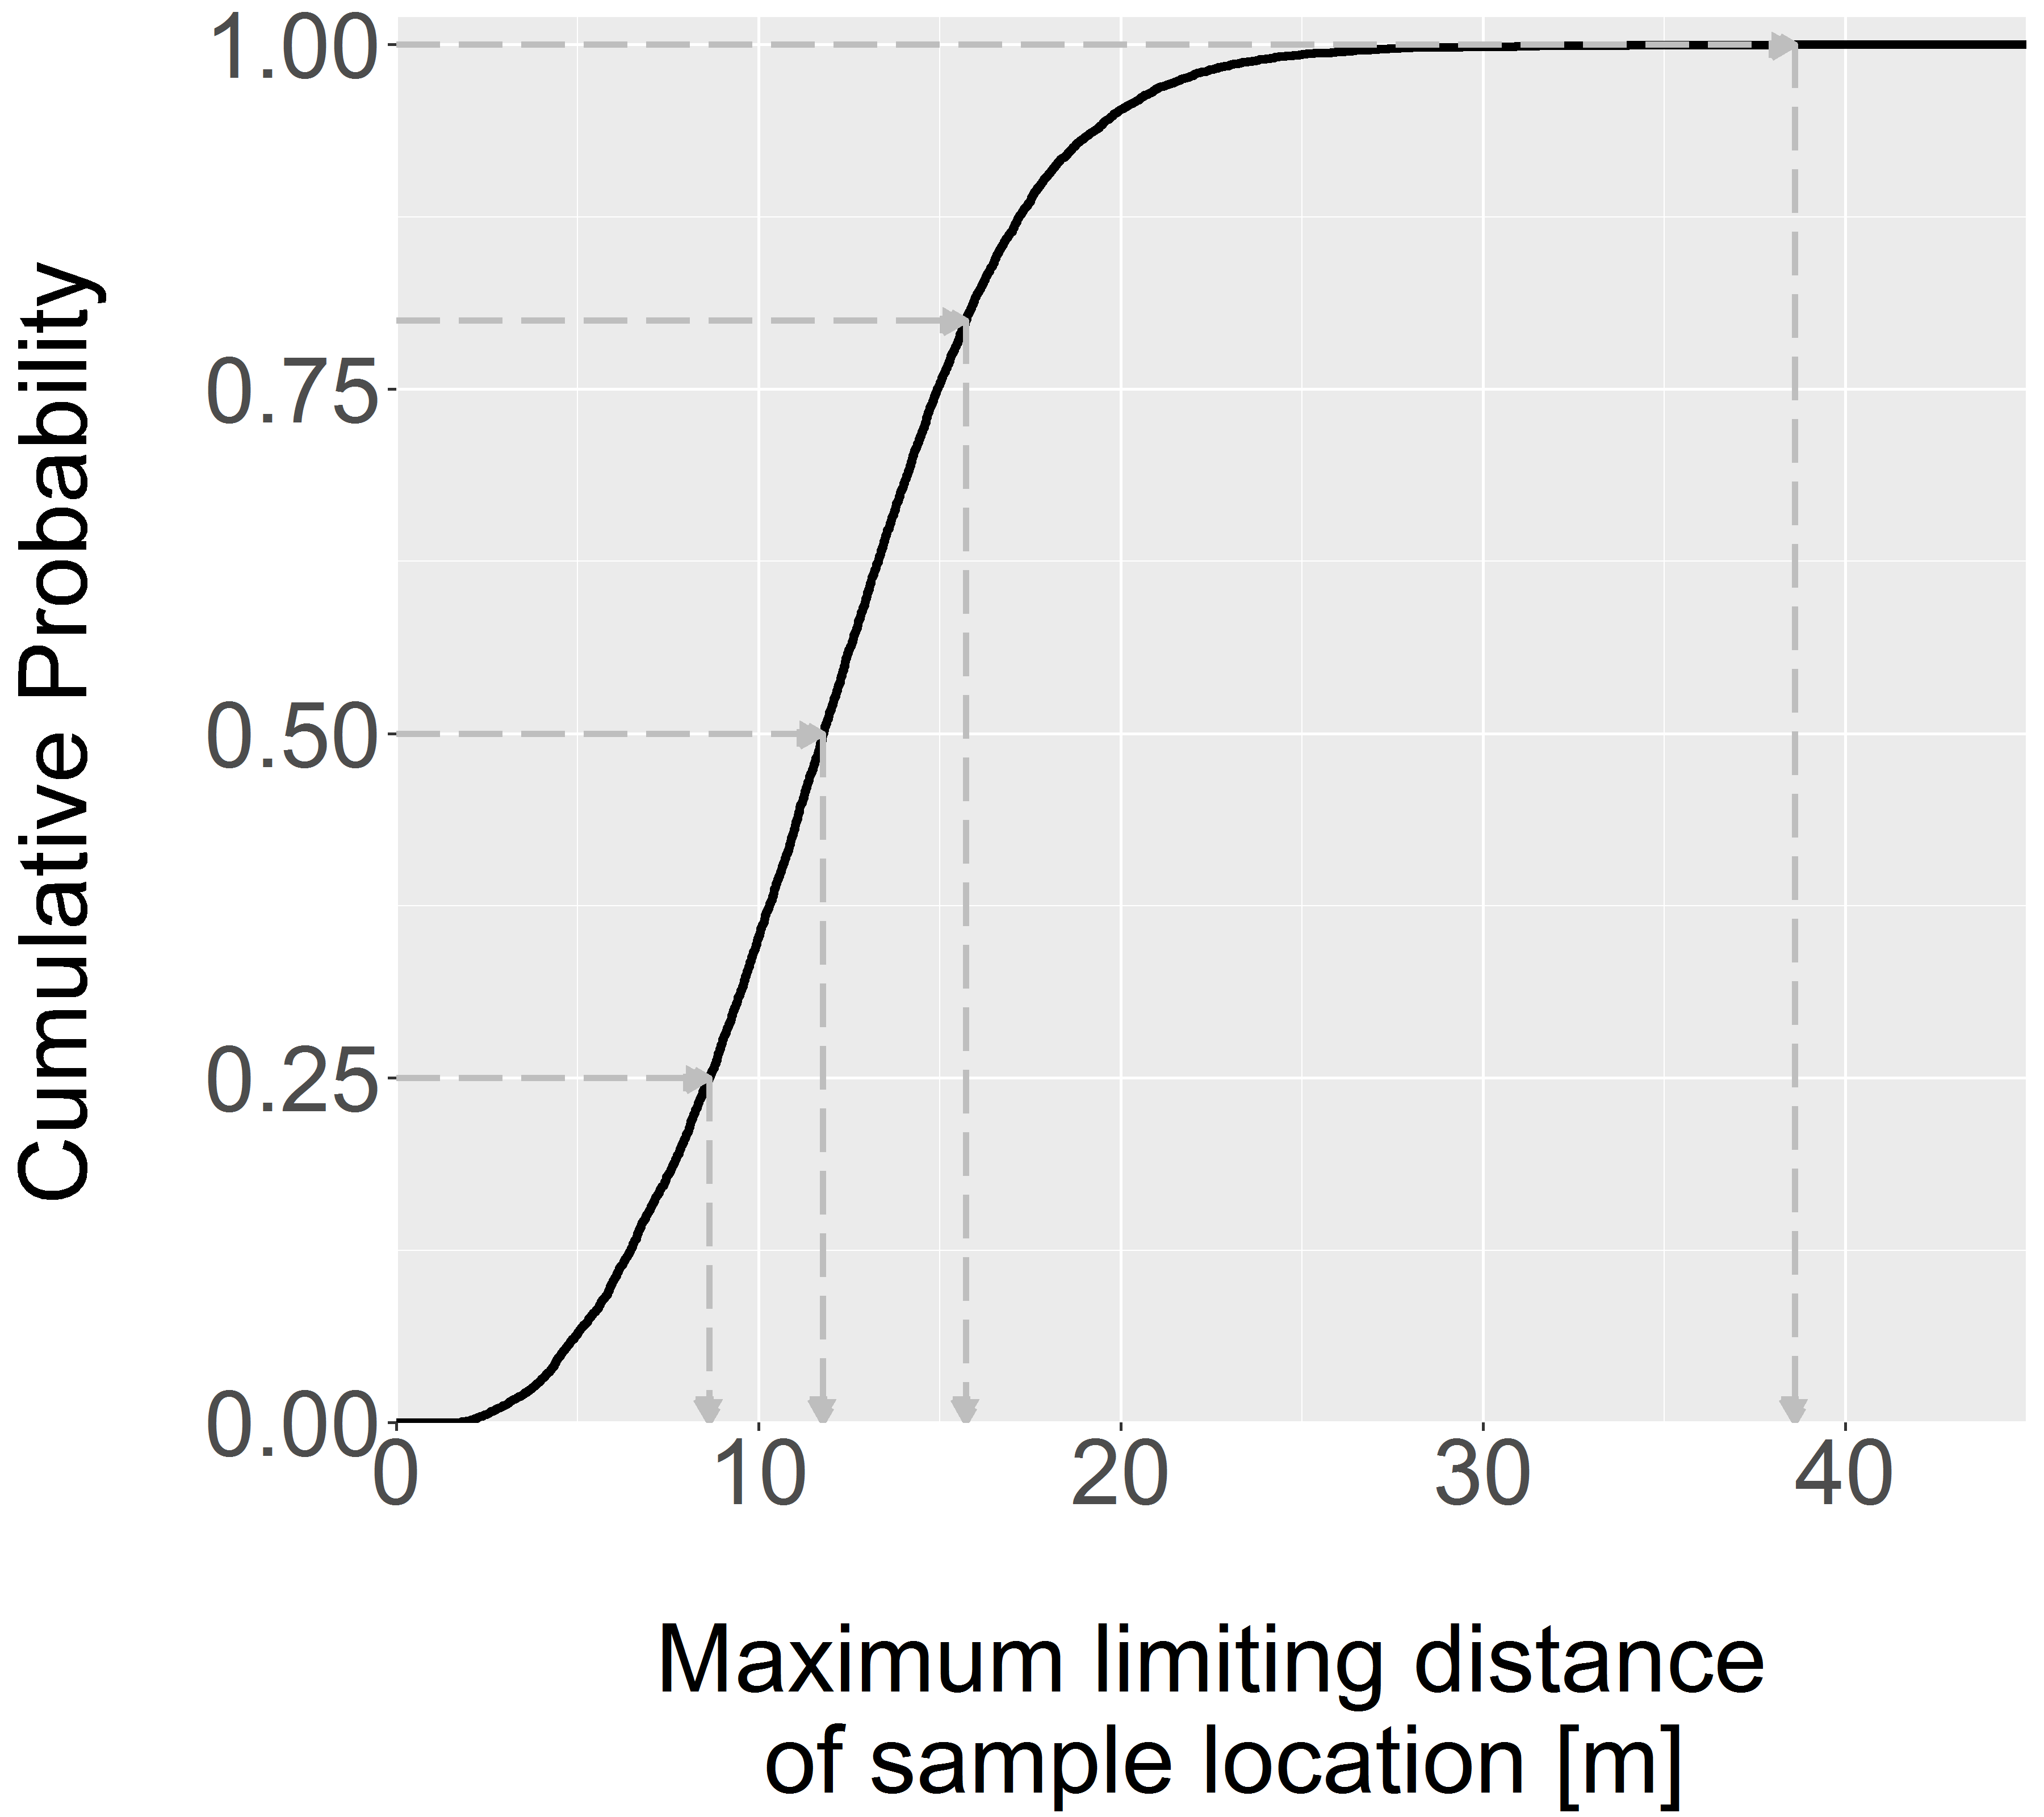
\includegraphics[width=0.36\textwidth]{cdf_maxri.png}%
  }\par\medskip
\subcaptionbox{Circular supports used to extract explanatory variables around sample locations. \textit{Dash dot dot line}: q100, \textit{dash dot line}: q80, \textit{dot dot line}: q50, \textit{dot line}: q25, \textit{solid line}: individual support, \textit{triangles}: sample trees \label{fig:sf2}}{
  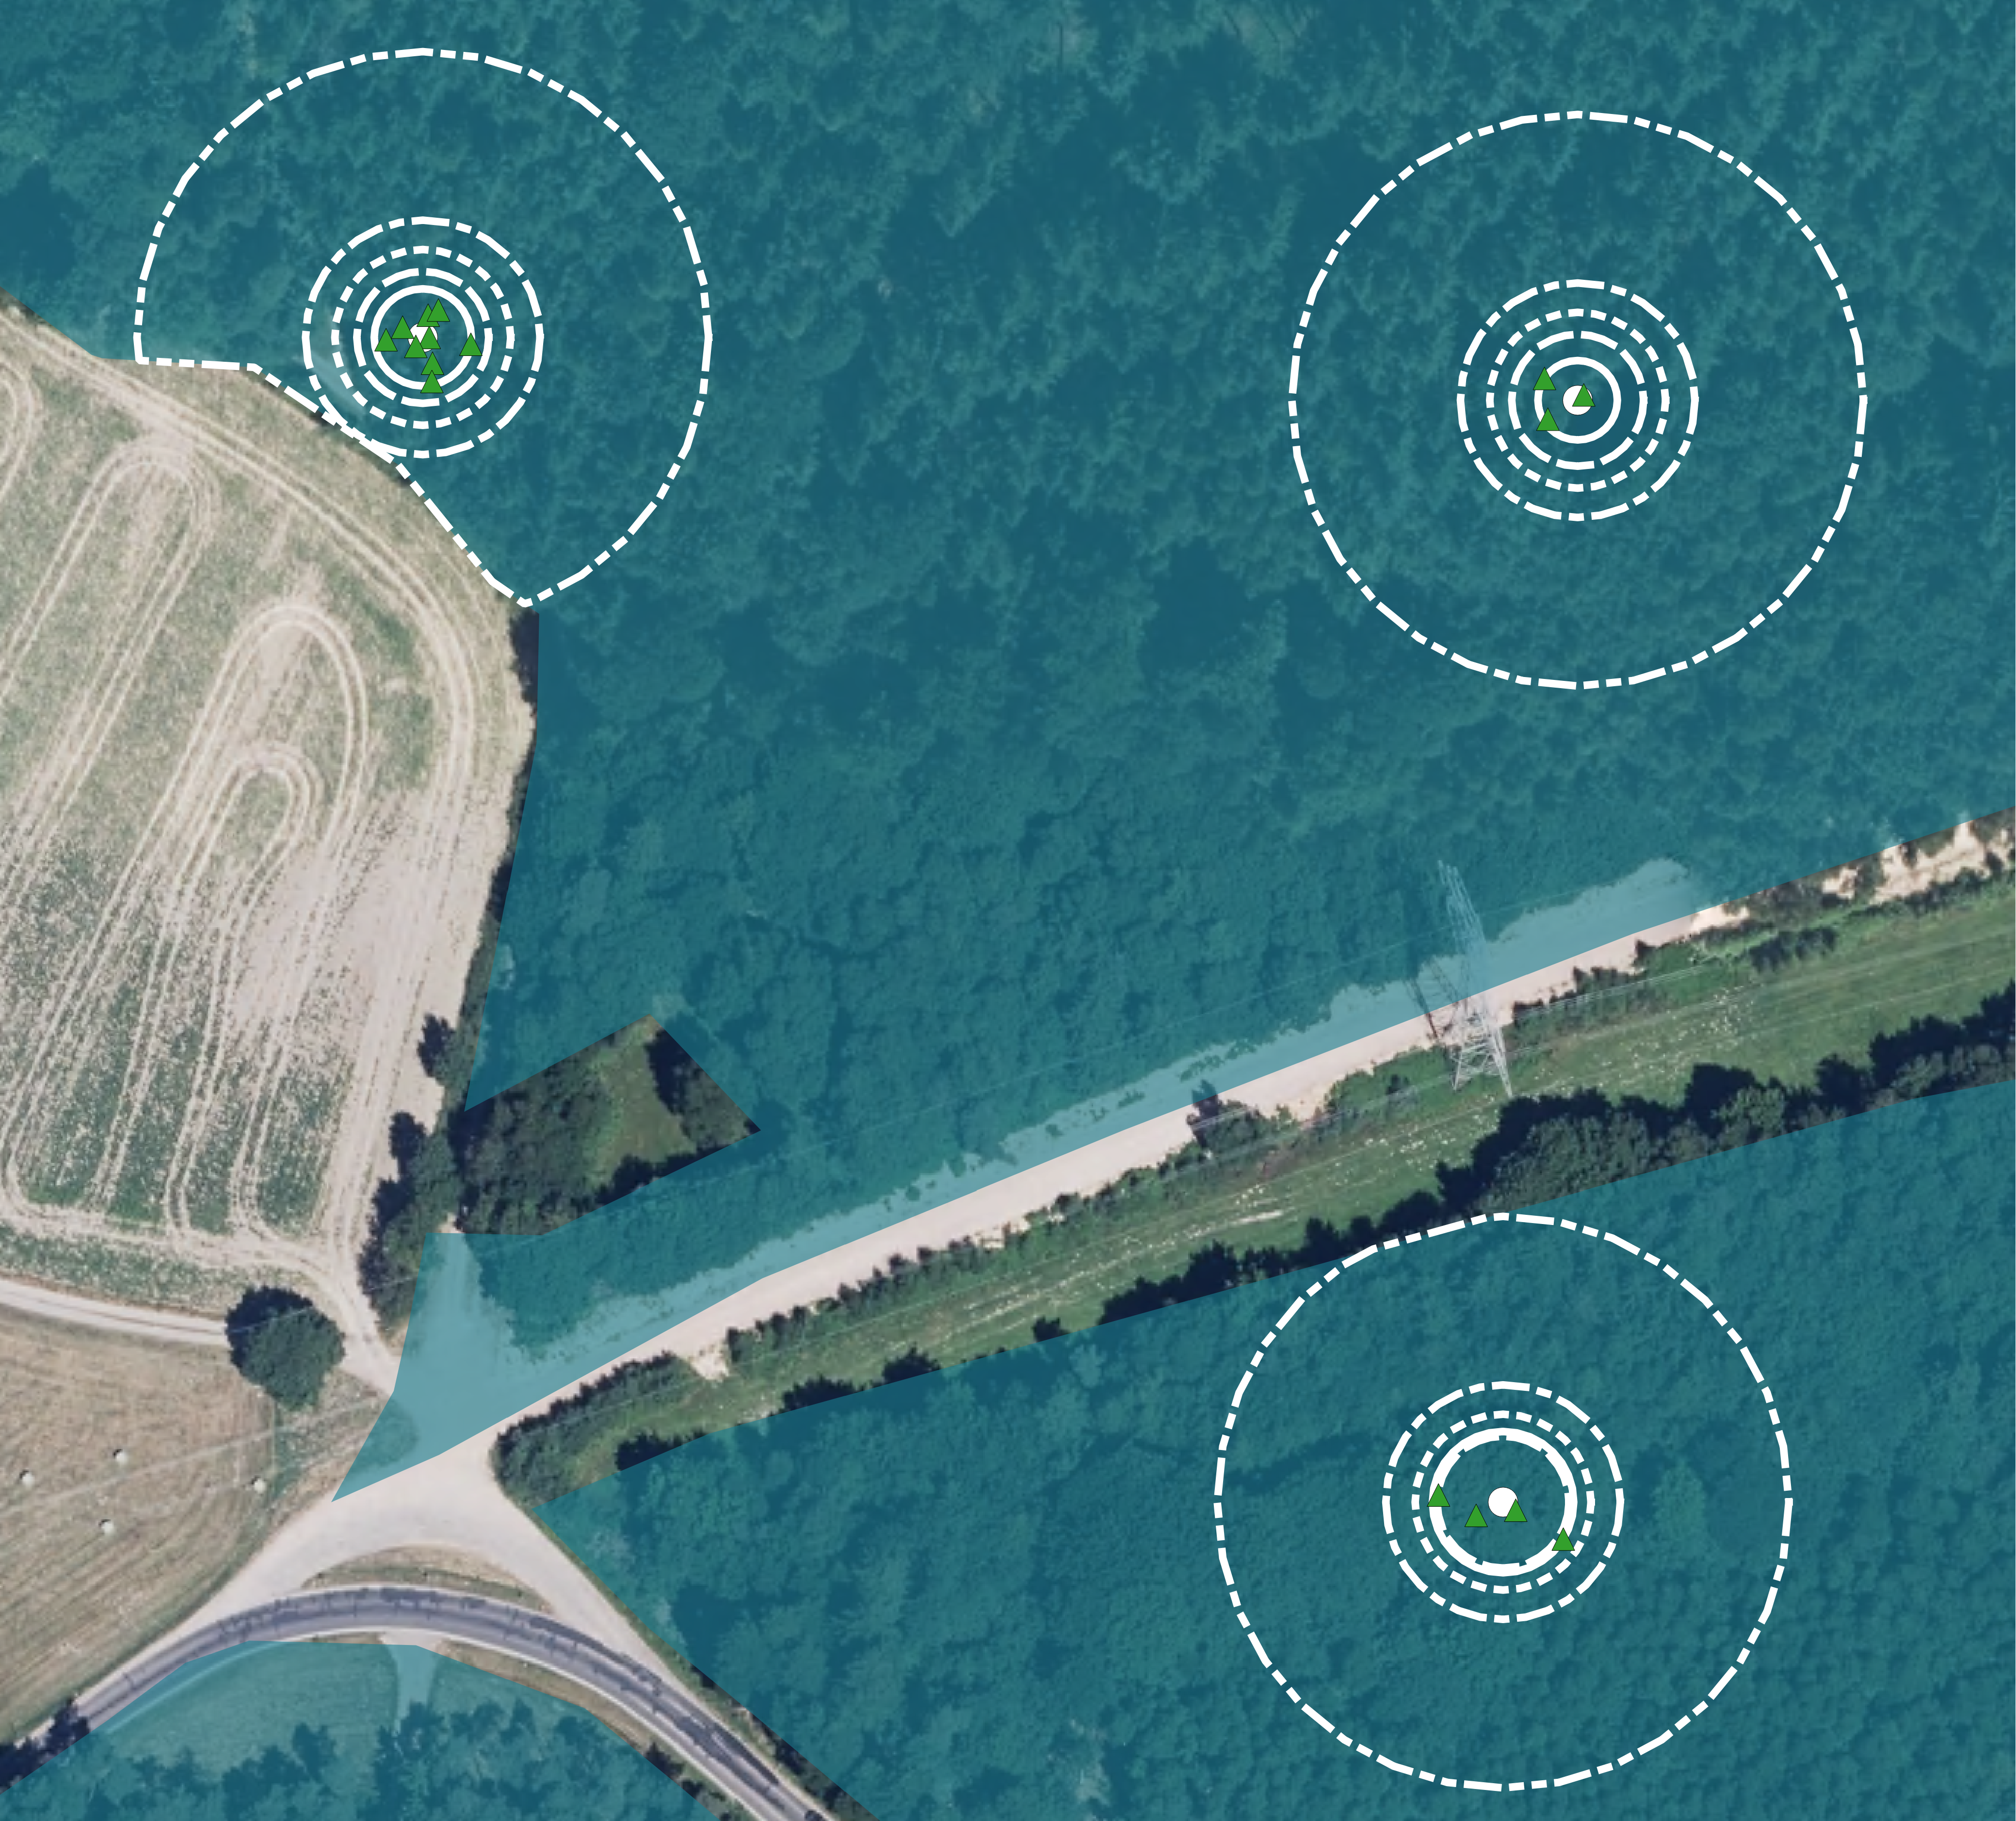
\includegraphics[width=0.36\textwidth]{choice_of_support.png}
  }\par\medskip
\caption{Identification (\textit{a}) and visualization (\textit{b}) of potential supports used for calculating the predictor variables on plot level}
\label{fig:tspec_supps}
\end{figure}


% ----------------------------------------------------------------------- %
% ----------------------------------------------------------------------- %
\subsection{\changed{Model Building and Evaluation}}
\label{sec:modval}

\changed{In order to judge the quality of the \textit{treespecies} variable, the user's accuracy for each classified species category and the overall accuracy of the classification scheme was calculated based on the confusion matrix \citep{congalton2008}. As reference data, we calculated the actual main plot tree species by applying the respective threshold to the sample trees of each sample plot.} The classification accuracy was evaluated for all support sizes for both the calibrated and the uncalibrated \textit{treespecies} variables. The measures of the regression model accuracy using both CHM- and $treespecies$ variables were defined as the 10-fold cross-validated root mean square error (\rmsecv{}, equation \ref{eq:RMSE}) and the adjusted coefficient of determination (\adjrsq{}) of the multiple linear regression model defined in equation \ref{eq:chmtspec_fullmod_term}. Additionally, we considered the interaction terms \textit{meanheight}:\textit{treespecies}, \textit{meanheight$^{2}$:treespecies}, \textit{meanheight}:\textit{ALSyear}, \textit{stddev}:\textit{ALSyear} and \textit{meanheight}:\textit{stddev} and performed a variable selection based on the Akaike Information Criterion (AIC) \citep{Akaike2011} in order to minimize the number of variables in the model. Due to a pronounced unbalanced design in the \textit{treespecies}-\textit{ALSyear} strata (Online Resource 2), no interaction between \textit{treespecies} and \textit{ALSyear} was possible. We evaluated the model for all support combinations, considering the use of individual support sizes for each auxiliary information, using both the calibrated and the uncalibrated \textit{treespecies} variable. The calibration model (section \ref{sec:tspecclass}) for the \textit{treespecies} variable was recalculated for each respective support-threshold setting.\par

206 sample plots included no sample trees and the timber volume density $Y(x)$ was thus set to \textit{zero}. These \textit{zero-plots} were removed from the modeling dataset since they acted as leverage points in cases where the ALS height metrics were recorded long before the terrestrial survey. Together with the missing tree species information (section \ref{sec:tspecclass}), the modeling dataset $s$ was limited to $n$=\changed{5171} observations.

\begin{subequations}\label{eq:RMSE}
	\begin{align}
	RMSE &= \sqrt{\frac{\sum_{x \in s}\big(\hat{Y}(x)-Y(x)\big)^2}{n}} \label{eq:RMSEa}\\
	RMSE\% &= \frac{RMSE}{\frac{1}{n}\sum_{x \in s}Y(x)}	\label{eq:RMSEb}
	\end{align}
\end{subequations}


\begin{equation} \label{eq:chmtspec_fullmod_term}
\begin{split}
Y(x) = &\beta_{0} + \beta_{1}*meanheight + \beta_{2}*meanheight^{2} + \\ 
&\beta_{3}*stddev + \\
&\beta_{4}*ALSyear_1 + ... + \beta_{12}*ALSyear_9 + \\
&\beta_{13}*treespecies_1 + ... + \beta_{18}*treespecies_6 + \varepsilon(x)
\end{split}
\end{equation}

